\documentclass{minimal}
\usepackage{amsmath}
\usepackage{amssymb}
\usepackage{tikz}
\usetikzlibrary{trees}
\tikzstyle{coordaxis}=[draw=red!50!black, thick, ->]
\tikzstyle{mapping}=[draw=blue!50!black, thick, ->]
\tikzstyle{connect}=[draw=green!50!black, thick, ->]
\newcommand{\sR}{\mathbb{R}}


\begin{document}

%	grow=down,
%    every node/.style={draw, circle, thin},
%    edge from parent/.style={-latex, thick, draw}
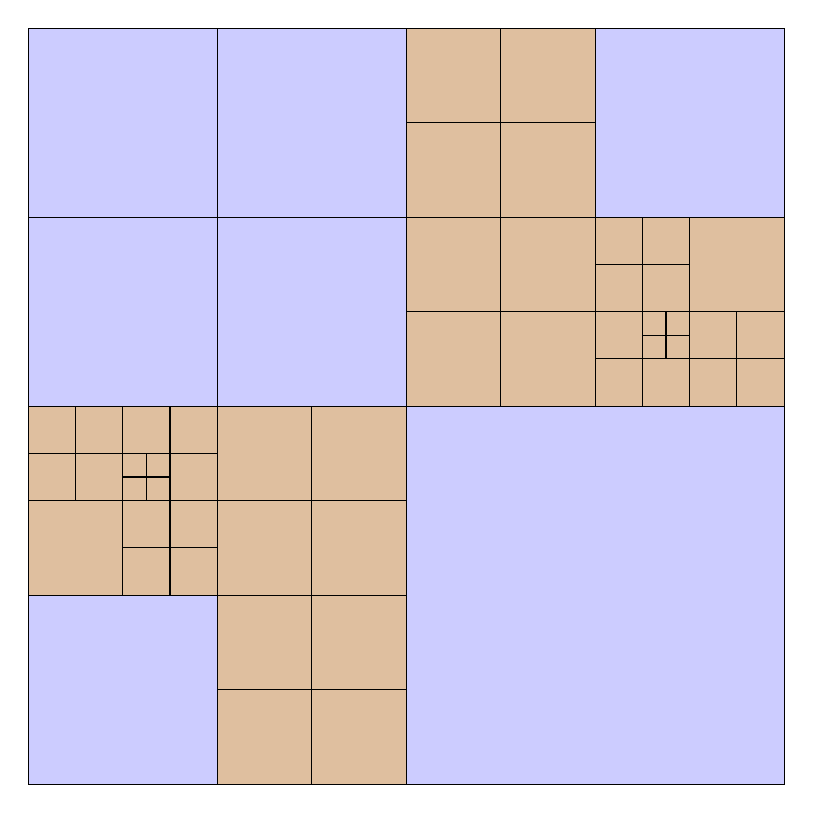
\begin{tikzpicture}[scale=0.6]

\draw[fill=blue!20] (0,8) rectangle +(8,8);
\draw[fill=blue!20] (8,0) rectangle +(8,8);
\draw[fill=blue!20] (0,0) rectangle +(4,4);
\draw[fill=blue!20] (12,12) rectangle +(4,4);

\draw[fill=brown!50] (4,0) rectangle +(4,4);
\draw[fill=brown!50] (0,4) rectangle +(4,4);
\draw[fill=brown!50] (4,4) rectangle +(4,4);
\draw[fill=brown!50] (8,8) rectangle +(4,4);
\draw[fill=brown!50] (8,12) rectangle +(4,4);
\draw[fill=brown!50] (12,8) rectangle +(4,4);

%Draw the initial octree
\draw[step = 8] (0,0) grid (16,16);
\draw[step = 4] (8,8) grid(16,16);
\draw[step = 4] (0,8) grid(8,16);
\draw[step = 2] (0,4) grid(4,8);
\draw[step = 2] (4,4) grid (8,8);
\draw[step = 2] (4,0) grid (8,4);
\draw[step = 1] (2,4) grid (4,8);    	
\draw[step = 1] (0,6) grid (2,8);
\draw[step = 0.5] (2,6) grid (3,7);

\draw[step = 2] (8,8) grid(12,16);
\draw[step = 2] (12,8) grid (16,12);
    	    	
\draw[step = 1] (12,8) grid (14,12);
\draw[step = 1] (14,8) grid (16,10);
\draw[step = 0.5] (13,9) grid (14,10);    	    	    	    	
    	    	    	    	
\end{tikzpicture}




%sibling distance=2cm,
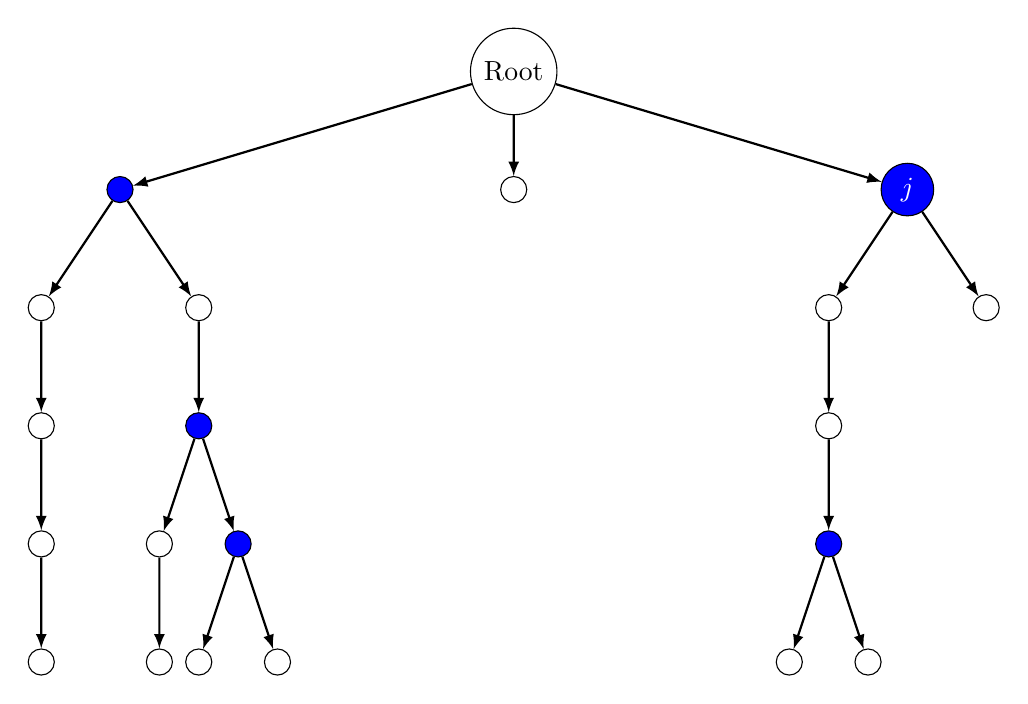
\begin{tikzpicture}[level distance=1.5cm, grow=down,
    every node/.style={draw, circle, thin},
    edge from parent/.style={-latex, thick, draw},
 level 1/.style={sibling distance=5cm},
 level 2/.style={sibling distance=2cm},
 level 3/.style={sibling distance=1.cm}
 ]
\node (P) {Root}
    child {node [fill=blue] (C1) {}
        child {node (T) {}
 	        	 child { node (TTT) {}
                      child {node (TTTT) {}
                             child {node (TTTTT) {}
                                   }
                             }
                       }
               }
        child {node (U) {}
 	        	 child { node [fill=blue] (TTT) {}
                      child {node (TTTT) {}
                             child {node (TTTTT) {}
                                   }
                             }                                   
                            child {node [fill=blue] (TTTTU) {}
                                  child {node (TTTTU1) {}}
                                  child {node (TTTTU2) {}}
                                   }
                        }         
                }
      }
    child {node (C2) {}}
%    child {node (C3) {}}
   child {node [fill=blue, text=white] (C4) {$j$}
        child {node (T) {}
	        child {node (TT) {}
	        	 child { node [fill=blue] (TTT) {}
                      child {node (TTTT) {}}
                       child {node (TTTU) {}}
                       }          
              }                   
        }
        child {node (U) {}}
    };

\path (P) -- coordinate[midway] (PQ) (C1);
\path (P) -- coordinate[midway] (PR) (C2);

%\draw (PQ) to[bend right=22] (PR);
\end{tikzpicture}

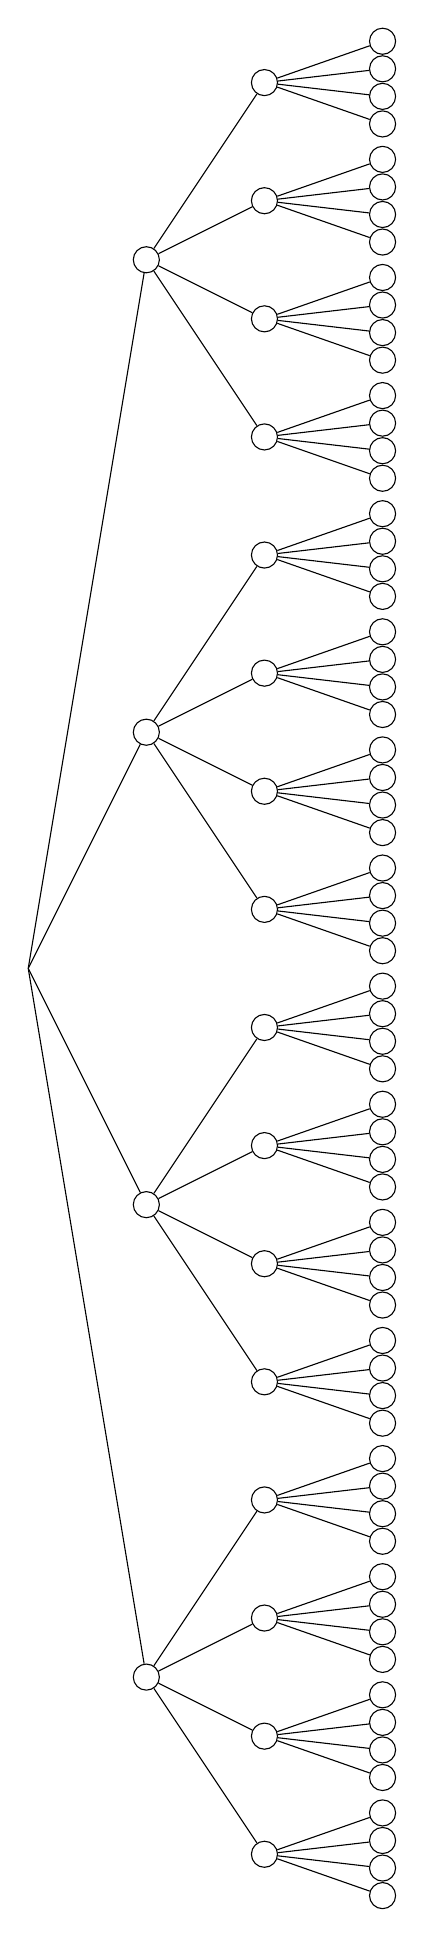
\begin{tikzpicture}
  [level distance=30mm, %level/.style={sibling distance=36mm/#1}]
    every node/.style={draw, circle, thin},
%        edge from parent/.style={-latex, thick, draw},
 level 1/.style={sibling distance=12cm},
 level 2/.style={sibling distance=30mm},
 level 3/.style={sibling distance=7mm},
 scale=0.5, rotate=90 ]
 \coordinate
    child foreach \x in {0,1,2,3}  {node{}
      {child foreach \y in {0,1,2,3}  {node{}
        {child foreach \z in {0,1,2,3} {node{}}} }}};
\end{tikzpicture}

\begin{tikzpicture}
%\node {root} child [red] foreach \name in {1,2} {node {\name}}
\end{tikzpicture}
\end{document}